\section{Effect of changing the classification threshold}
\lb{sec:thres}


In this section we study the effect of changing the threshold



\begin{figure*}[h]
\centering
\hspace*{-0.5cm}
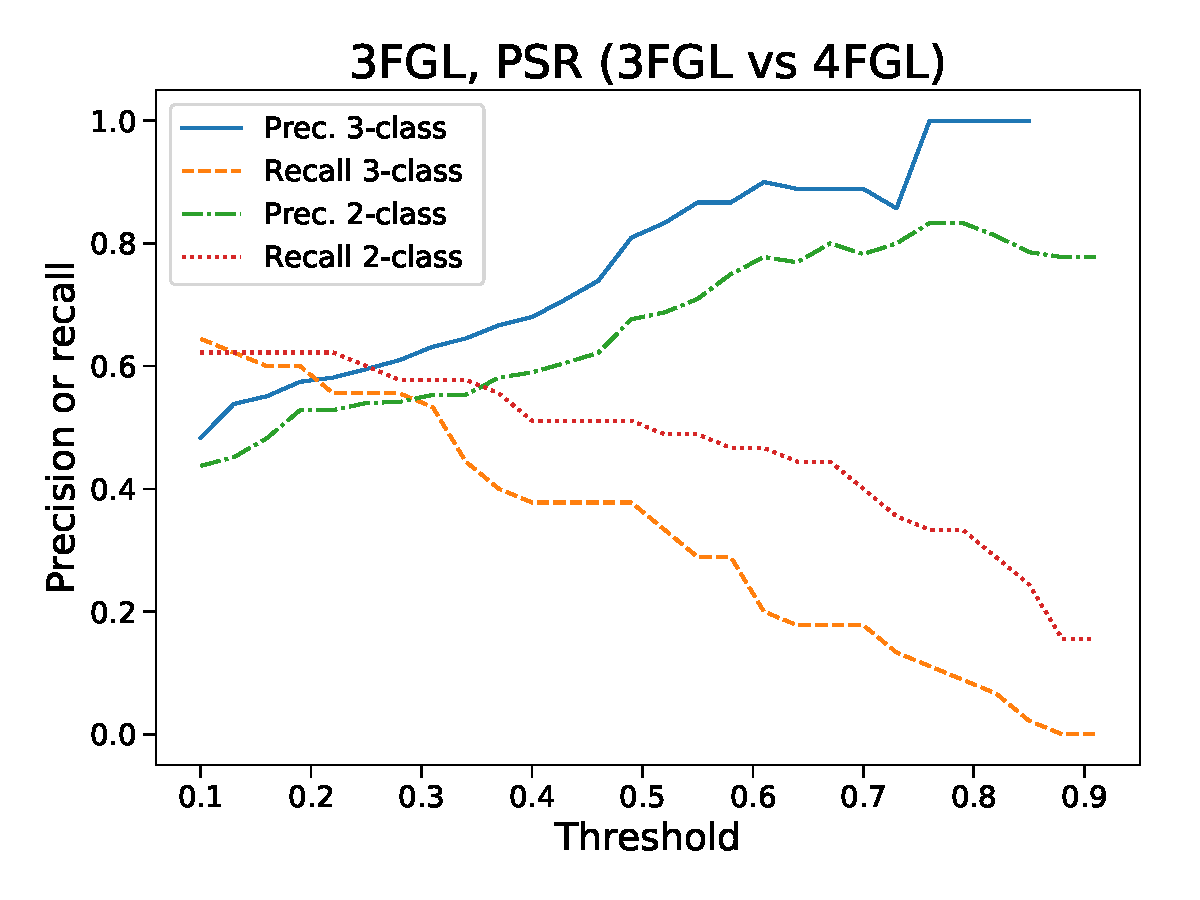
\includegraphics[width=0.45\textwidth]{plots/thresholds/thresholds_prec_recall_3FGL_vs_4FGL-DR2_PSR.pdf}
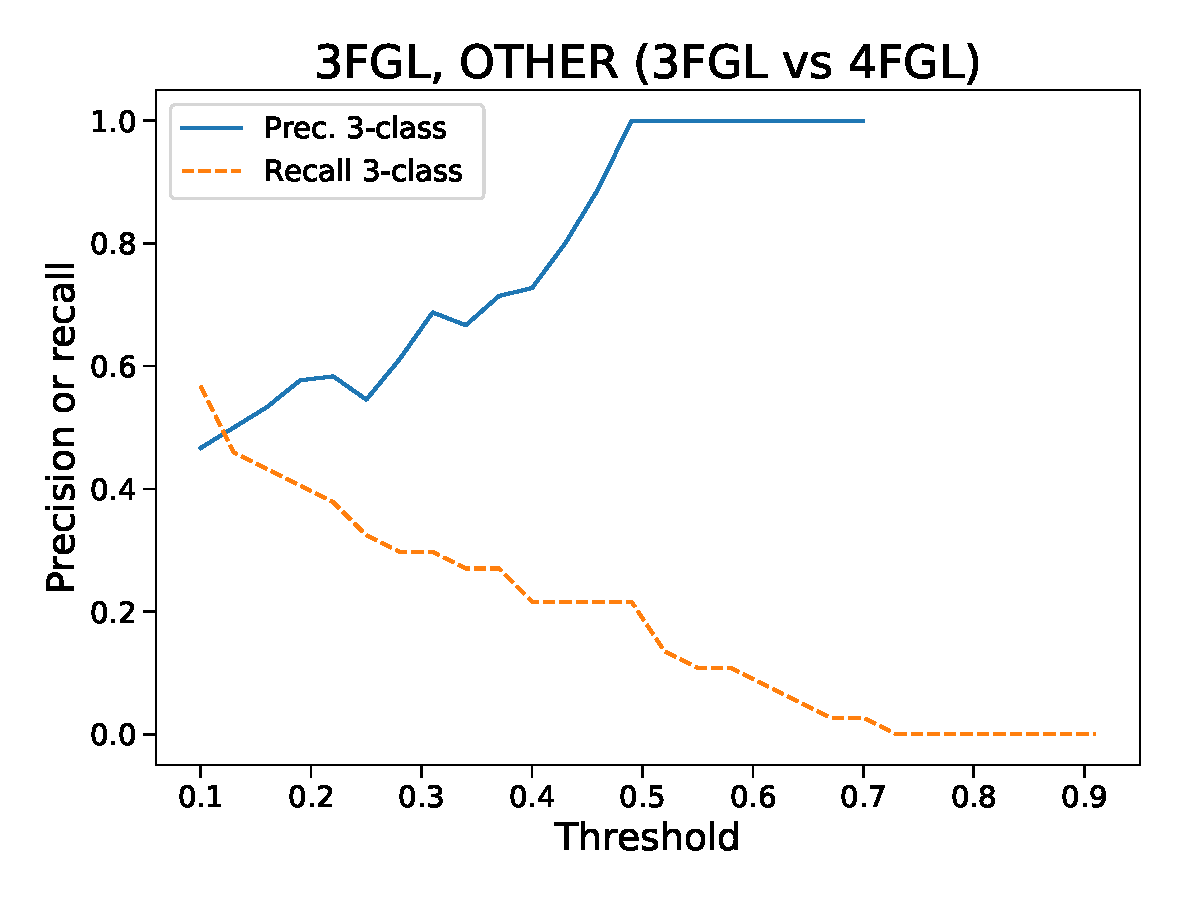
\includegraphics[width=0.45\textwidth]{plots/thresholds/thresholds_prec_recall_3FGL_vs_4FGL-DR2_OTHER.pdf}
	%\hspace*{-0.5cm}
%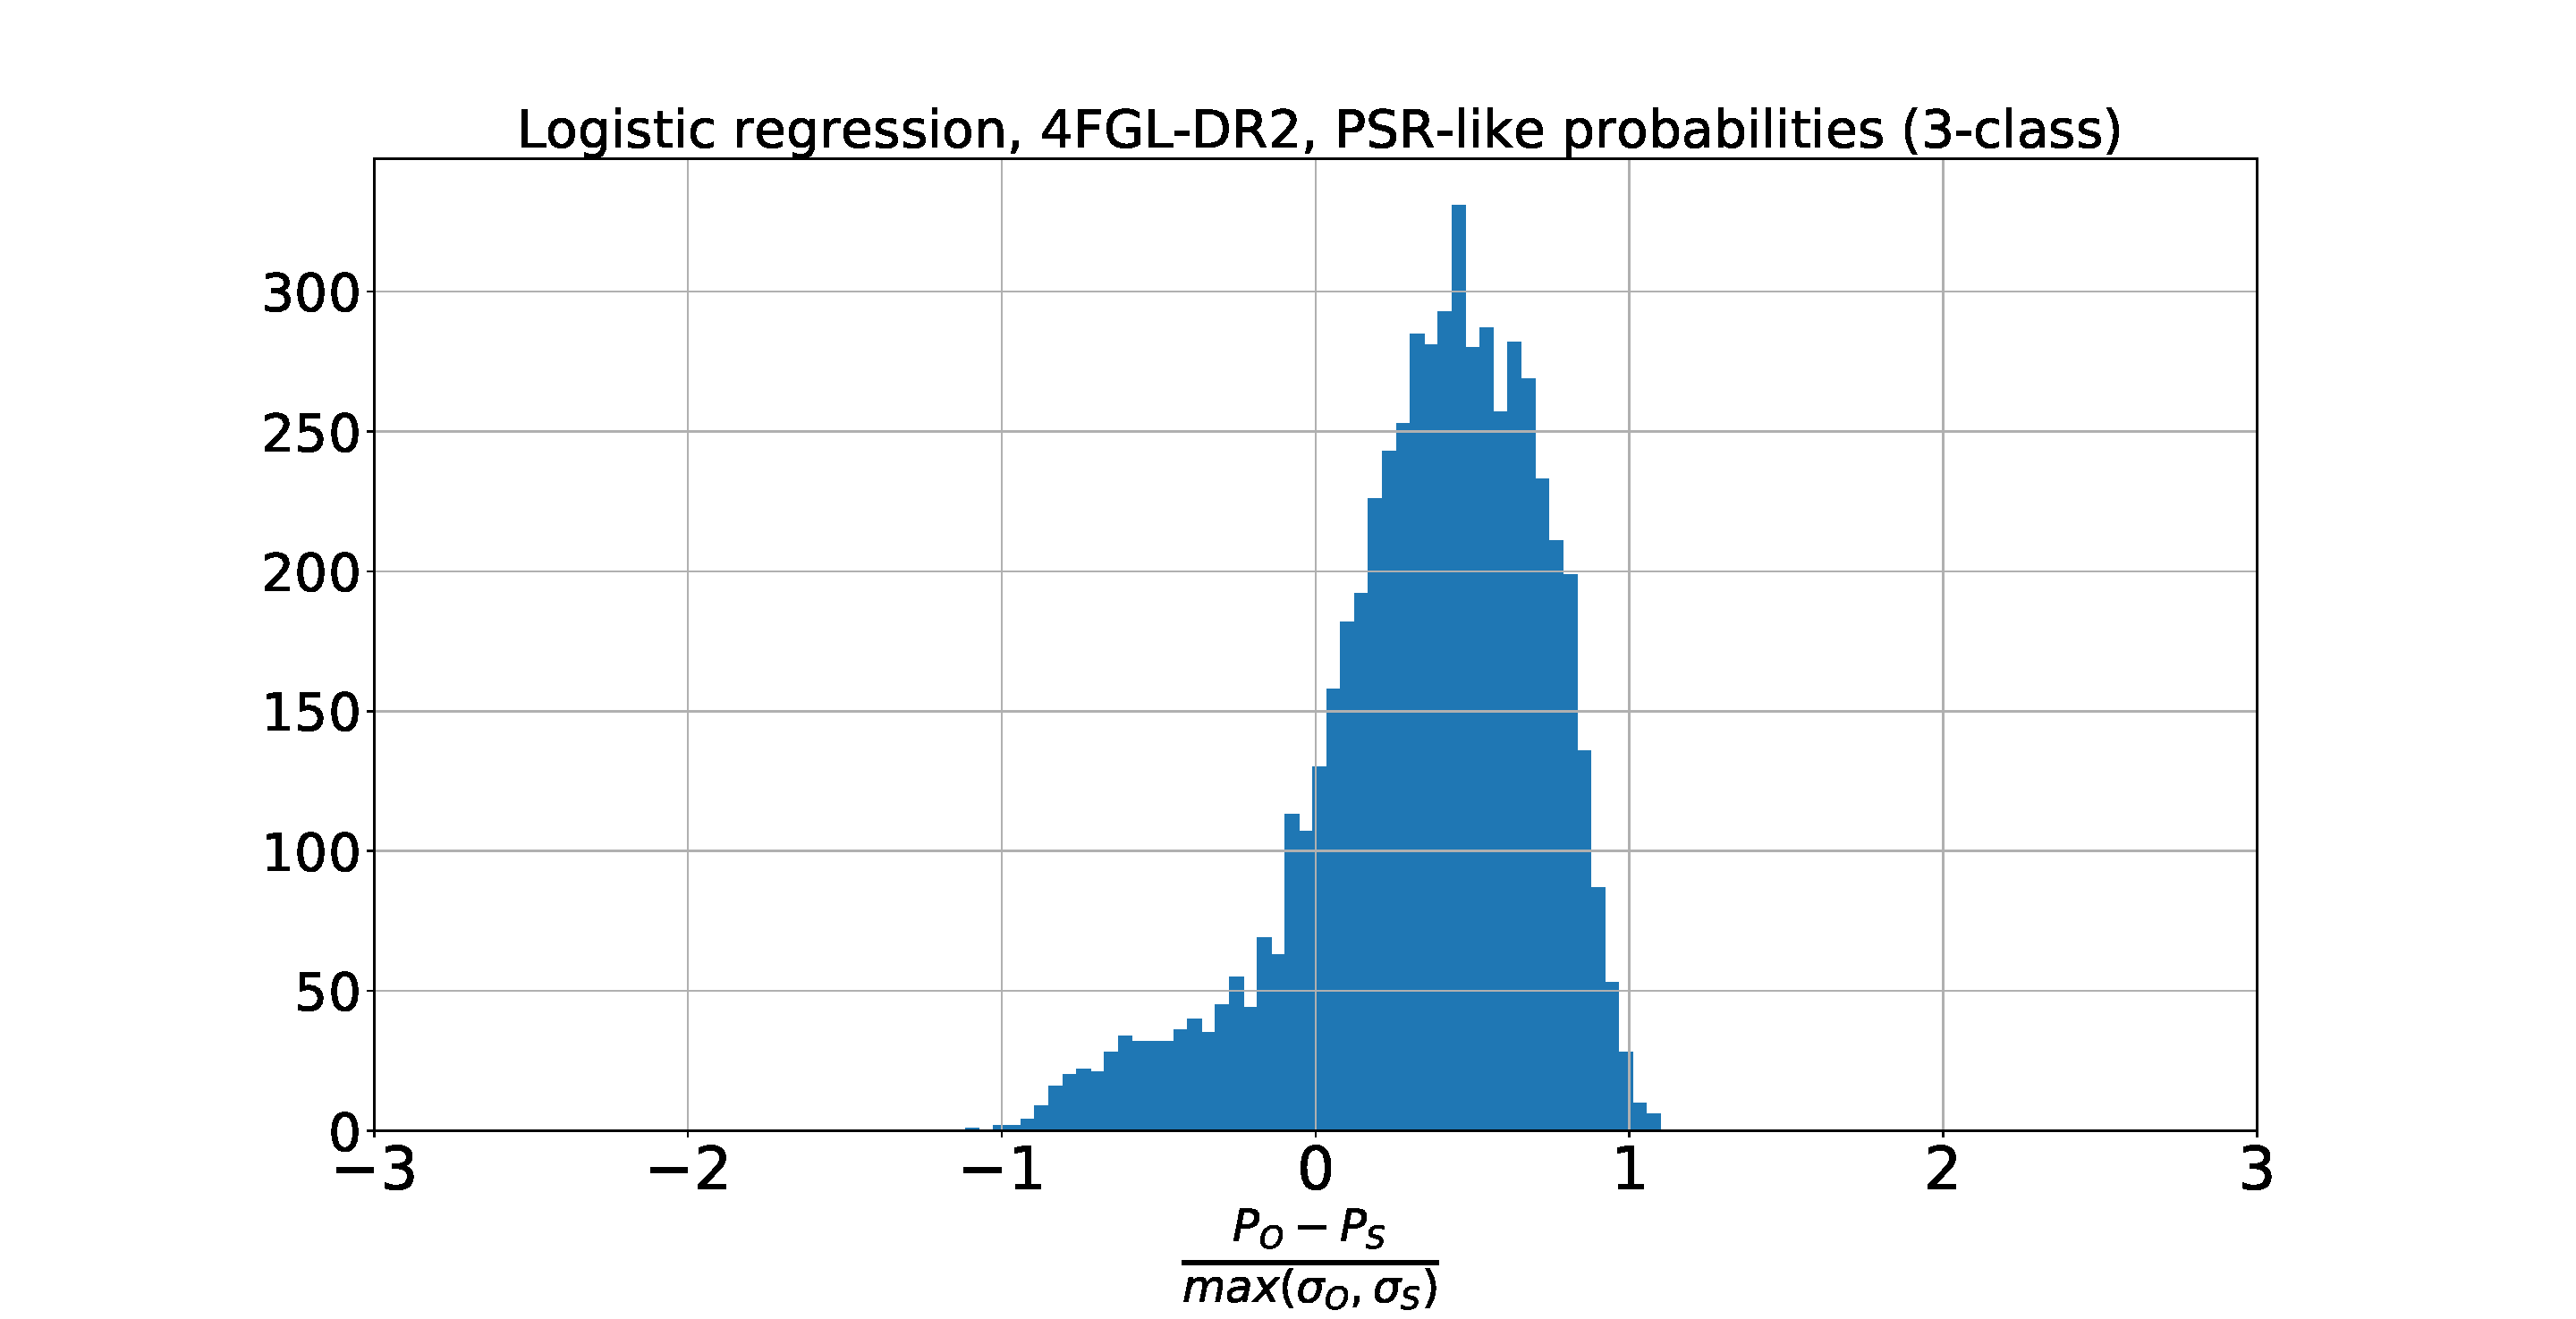
\includegraphics[width=0.55\textwidth]{plots/hist_diff_smote_LR_4FGL-DR2_3class.pdf}
\caption{Effect of thresholds.
}
\label{fig:thres_3_vs_4}
\end{figure*}


\begin{figure*}[h]
\centering
\hspace*{-0.5cm}
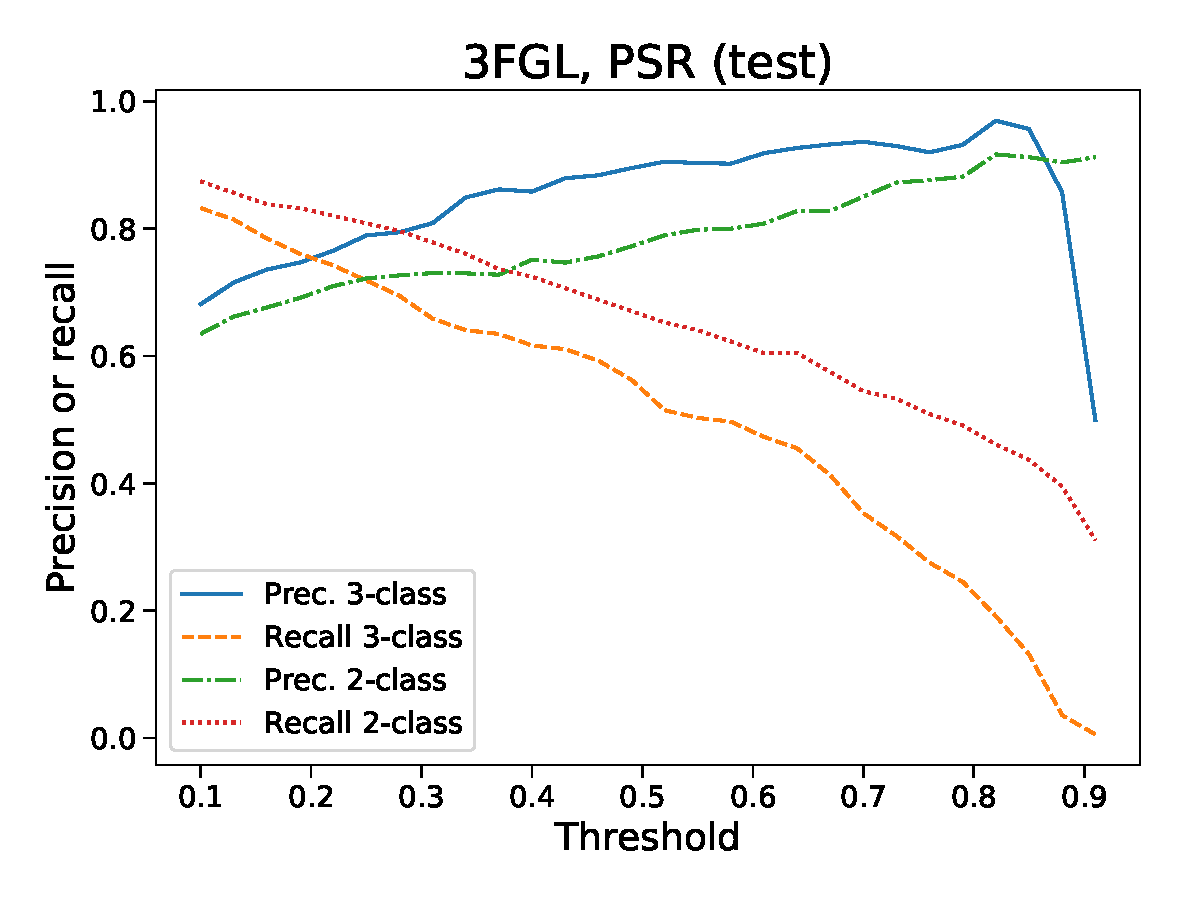
\includegraphics[width=0.45\textwidth]{plots/thresholds/thresholds_prec_recall_3FGL_PSR.pdf}
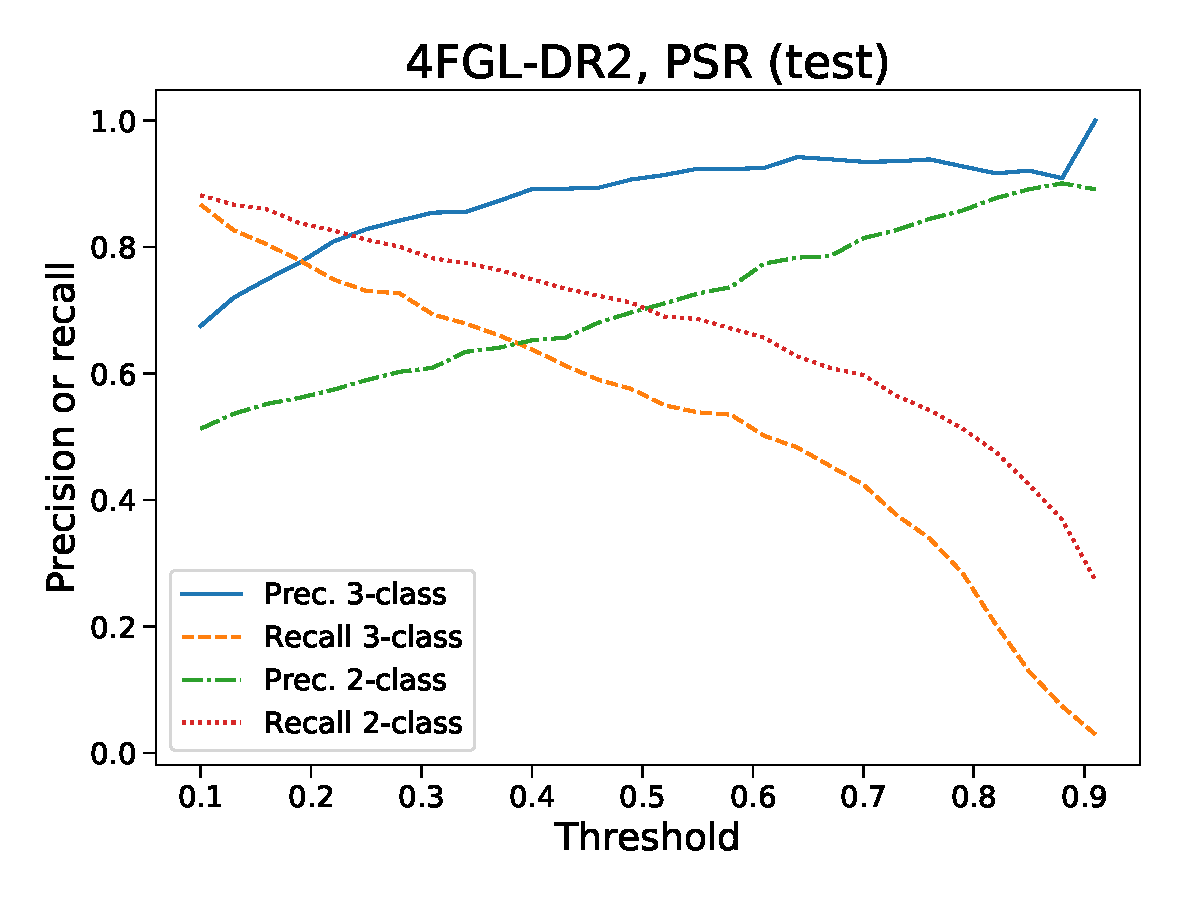
\includegraphics[width=0.45\textwidth]{plots/thresholds/thresholds_prec_recall_4FGL-DR2_PSR.pdf} \\ 
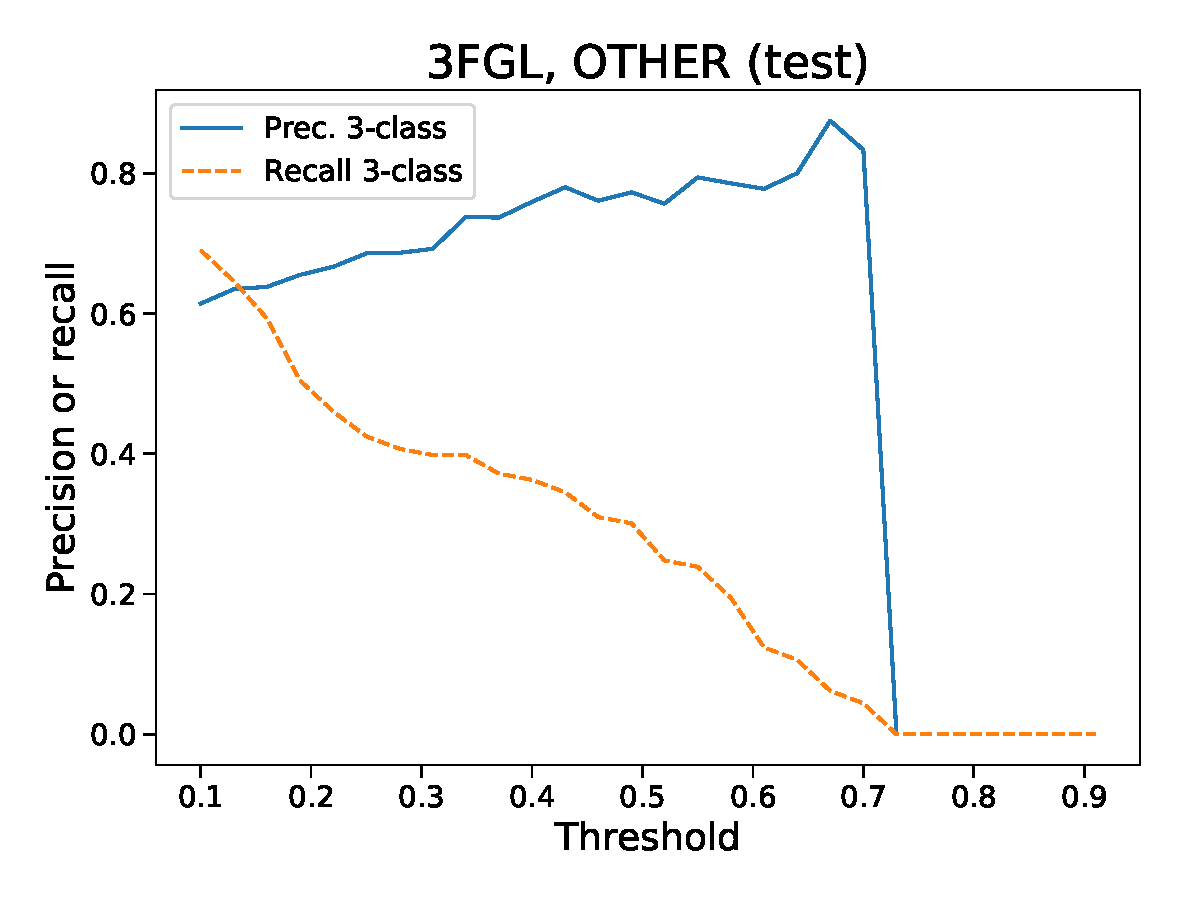
\includegraphics[width=0.45\textwidth]{plots/thresholds/thresholds_prec_recall_3FGL_OTHER.pdf}
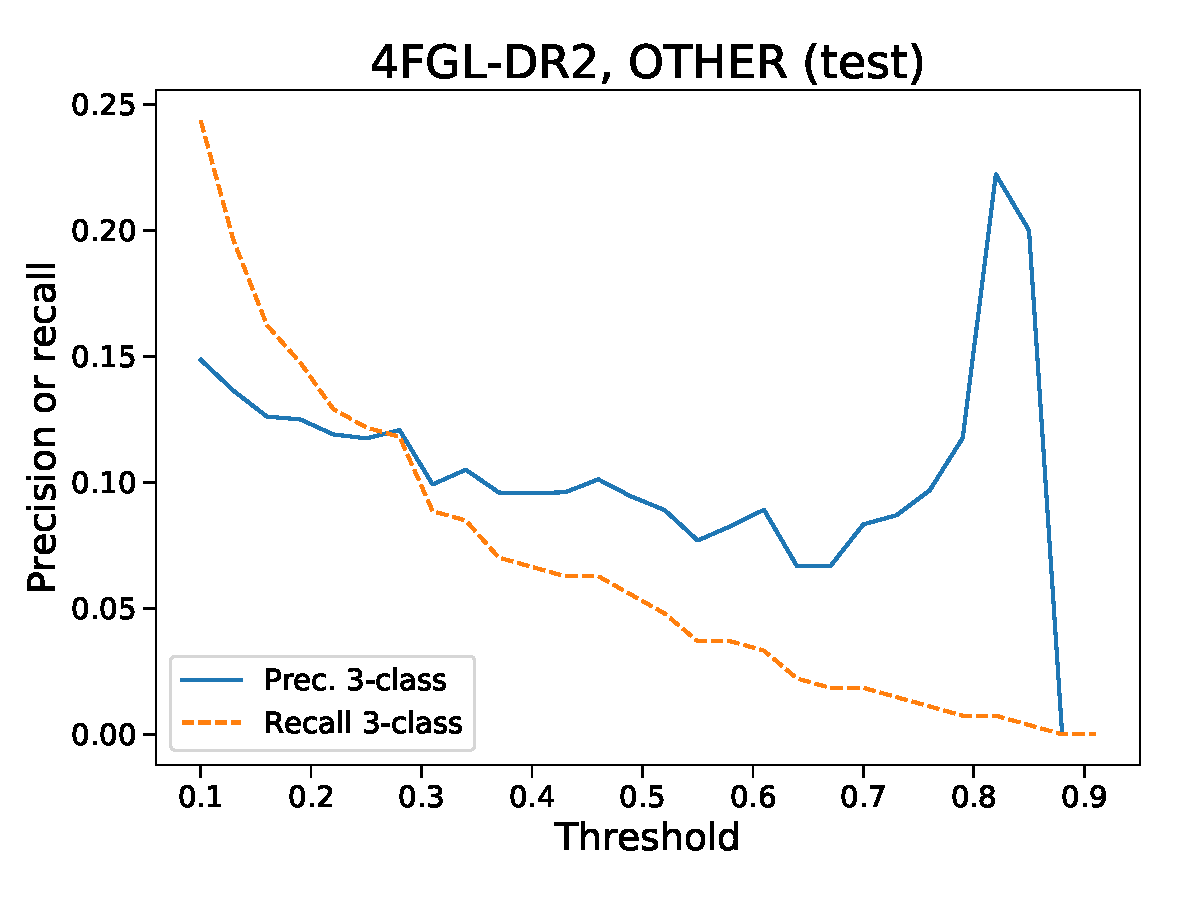
\includegraphics[width=0.45\textwidth]{plots/thresholds/thresholds_prec_recall_4FGL-DR2_OTHER.pdf}
	%\hspace*{-0.5cm}
%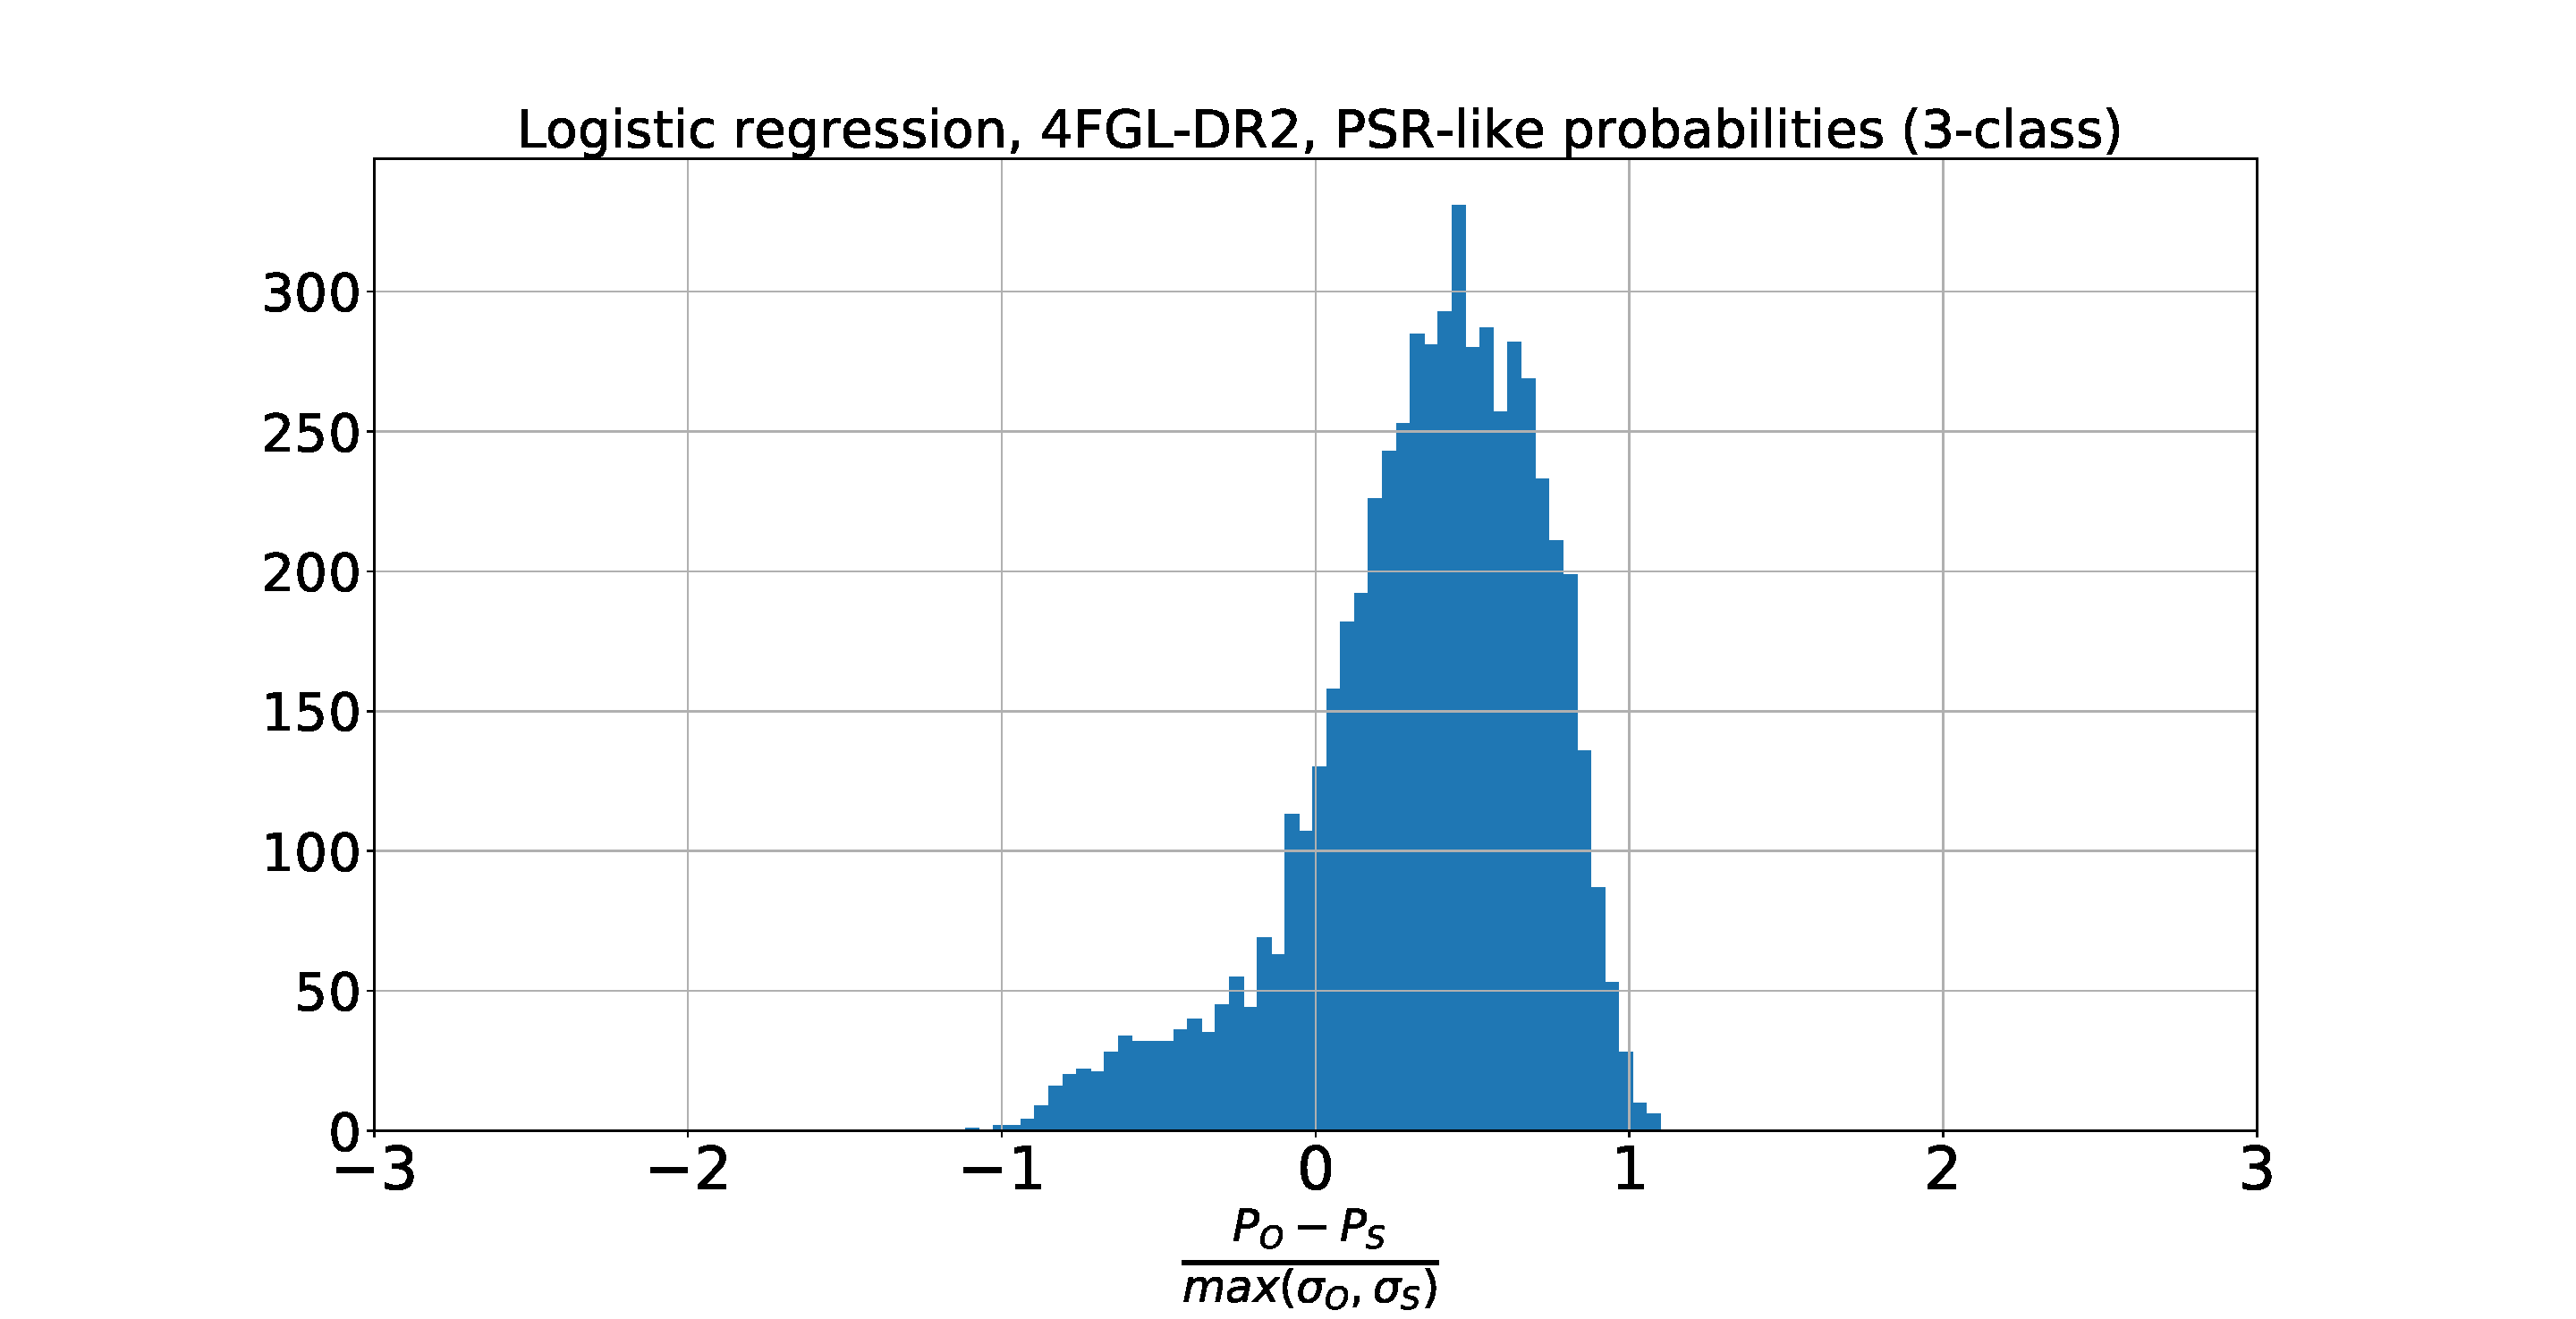
\includegraphics[width=0.55\textwidth]{plots/hist_diff_smote_LR_4FGL-DR2_3class.pdf}
\caption{Effect of thresholds.
}
\label{fig:thres}
\end{figure*}
